\subsection{Signs et feedbacks}

Pour aider à la compréhension du jeu, nous avons ajouter des signs et des feedbacks, sonores ou visuels.

\subsubsection{Signs}
    Un exemple de sign utilisé est les fissures sur les chaudrons. En fonction des points de vies du chaudron il apparaitra plus ou moins fissuré à l'écran (figure \ref{fig:sign}).

    \FloatBarrier
    \begin{figure}[h]
        \centering
        \begin{subfigure}[t]{0.45\textwidth}
            \centering
            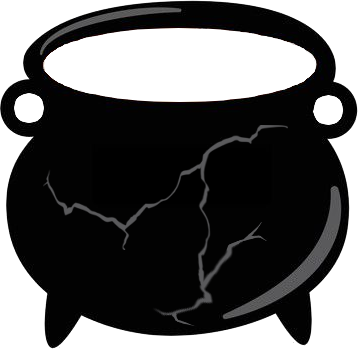
\includegraphics[width=\textwidth]{image/chaudron/chaudron2.png}
            \caption{Chaudron avec de légères fissures}
        \end{subfigure}
        \begin{subfigure}[t]{0.45\textwidth}
            \centering
            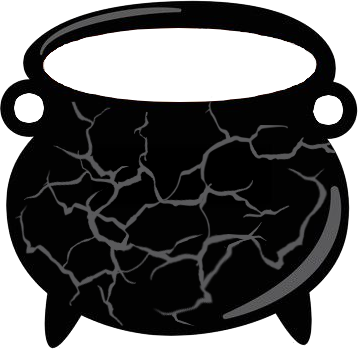
\includegraphics[width=\textwidth]{image/chaudron/chaudron3.png}
            \caption{Chaudron sur le point de se briser}
        \end{subfigure}
        \caption{Exemple de sign sur le chaudron}
        \label{fig:sign}
    \end{figure}


\subsubsection{Feedbacks}
    Les feedbacks sont les informations qui permettent au joueur d'avoir un retour sur une action qu'il a effectuée. Un exemple de feedback est l'animation lorsque le joueur prend des dégats (figure \ref{fig:feedback}). 
    
    \FloatBarrier
    \begin{figure}[h]
        \centering
        \begin{subfigure}[t]{0.45\textwidth}
            \centering
            
\includegraphics[width=\textwidth]{image/feedback/feedback1.png}
            \caption{Le joueur lors de son état normal}
        \end{subfigure}
        \begin{subfigure}[t]{0.45\textwidth}
            \centering
            
\includegraphics[width=\textwidth]{image/feedback/feedback2.png}
            \caption{Le joueur lorsqu'il prend un dégat}
        \end{subfigure}
        \caption{Exemple de feedback lorsque le joueur prend un dégat.}
        \label{fig:feedback}
    \end{figure}


\subsection{Les différents écrans}

Différents écrans ont été utilisés dans le jeu :
\begin{itemize}
    \item \textit{Menu principal}
    \item \textit{Réglages}
    \item \textit{Choix de partie}
    \item \textit{Combat}
    \item \textit{Fin de partie}
\end{itemize}
